\documentclass{report}
\usepackage[utf8]{inputenc}

% **********************************************************
% Document Settings                                        *
% **********************************************************
\usepackage{geometry}
% \geometry{a4paper, margin=2.5cm}
\geometry{a4paper,margin=2cm,top=2.5cm,headheight=16pt,headsep=0.1in,heightrounded}

\usepackage{graphicx}
% \graphicspath{{}}

\usepackage{minted}
% \usemintedstyle{emacs}

\usepackage{enumitem}
\usepackage{varwidth}
\usepackage{tasks}
\usepackage{multicol}
\usepackage{lscape}
\usepackage{tikz}
\usepackage{fancyhdr}


\pagestyle{fancy}
\fancyhf{}
\lhead{Data Structures and Algorithms}
\rhead{Suman Mondal}
% \lfoot{\href{https://github.com/thatsuman/knucse-assignment}{View on Github}}
\lfoot{\href{https://github.com/thatsuman}{github.com/thatsuman}}
\rfoot{Page \thepage}

\usepackage{hyperref}
\hypersetup{
colorlinks=true,
linkcolor=blue,
filecolor=magenta,
urlcolor=blue,
}
\urlstyle{same}

\usepackage{fontspec}
% \setromanfont{Source Sans Pro}
% \setmonofont{Cascadia Code PL}


% macros start here
\newcommand{\problem}[3]{
  \section{#3}
    \underline{{\LARGE Source Code :}}
    \inputminted[breaklines,fontsize=\Large]{c}{#1.c}
    \bigbreak
    \noindent
    \underline{{\LARGE Program Output :}}
    \bigbreak
    \noindent
    \includegraphics[height=2.1in]{#2}
% \newpage
}
\newcommand{\subproblem}[3]{
  \subsection{#3}
    \underline{\emph{\Large Source Code :}}
    \inputminted[breaklines]{c}{#1.c}
    \bigbreak
    \noindent
    \underline{\emph{\Large Program Output :}}
    \bigbreak
    \noindent
    \includegraphics{#2}
% \newpage
}
% macros end here

% **********************************************************

\begin{document}
%%%%%%%%%%%%%%%%%%%%%%55 If you use this cover separately %%%%%%%%%%%

% \documentclass[12pt]{report}
% \usepackage{graphicx}
% \usepackage{multicol}
% \usepackage{lscape}
% \usepackage{tikz}
% \usepackage{hyperref} 

% \begin{document}
% \centering
% 	{ \Large {\bfseries \textcolor{black}{{Data Structures and Algorithms}} \par}
% 	\vspace{1.5\baselineskip}
% 	{\normalsize An Assignment Work Submitted for the 3rd Semester \\ of Bachelor of Technology } \par
% 	\vspace{0.5\baselineskip}
% 	{\normalsize \textit{in} \par}
% 	\vspace{0.5\baselineskip}
% 	{\large \bf \textcolor{black}{Computer Science and Engineering (Data Science)} \par} 
% 	\vspace{0.5\baselineskip}
% 	{\normalsize \textit{by} \par}
% 	\vspace{0.5\baselineskip}
% 	{{\large {\bf \textcolor{black}{Suman Mondal} \\ Enrollment no.: KNU2200101}} \par}
% 	\vspace{1.5\baselineskip}
% 	{Under the guidance of \par}
% 	\vspace{0.5\baselineskip}
% 	{{\large \bf \textcolor{black}{Dr.Joydeep Dutta} \par}
% 	\vspace{0.5\baselineskip}
% 	{\begin{figure}[!h] 
% 			\centering
% 			
\includegraphics[width=40mm]{../../assets/Kazi_Nazrul_University_Logo.png} 
% 		\end{figure}
% 	}
% 	{\large \vspace*{1ex}
% 		\vspace{1\baselineskip}
% 		{\small \bf DEPARTMENT OF \MakeUppercase{Computer Science} \par}
% 		\vspace*{0.5ex}
% 		{\small \bf \uppercase{KAZI NAZRUL UNIVERSITY \par ASANSOL - 713340, WEST BENGAL} \par}
% 		\vspace{0.25\baselineskip}
% \end{document}

%%%%%%%%%%%%%%%%%%%%%%%%%%%%%%%%%%%%%%%%%%%%%%%%%%%%%%%%%%%%%%%%%%%%%%%%%%%%%%%%%%%%%%%%%%%%


\thispagestyle{empty}

\centering
	{ \huge {\bfseries \textcolor{black}{{Data Structures and Algorithms}} \par}
	\vspace{1.5\baselineskip}
	{\Large An Assignment Work Submitted for the 3rd Semester \\ of Bachelor of Technology } \par
	\vspace{1\baselineskip}
	{\Large \textit{in} \par}
	\vspace{1\baselineskip}
	{\LARGE \bf \textcolor{black}{Computer Science and Engineering (Data Science)} \par} 
	\vspace{1\baselineskip}
	{\Large \textit{by} \par}
	\vspace{1\baselineskip}
	{{\LARGE {\bf \textcolor{black}{Suman Mondal} \\ Enrollment no.: KNU2200101}} \par}
	\vspace{1.5\baselineskip}
	{Under the guidance of \par}
	\vspace{0.5\baselineskip}
	{{\LARGE \bf \textcolor{black}{Dr.Joydeep Dutta} \par}
	\vspace{0.5\baselineskip}
	{\begin{figure}[!h] 
			\centering
			
\includegraphics[width=40mm]{../../assets/Kazi_Nazrul_University_Logo.png} 
		\end{figure}
	}
	{\LARGE \vspace*{1ex}
		\vspace{1\baselineskip}
		{\large \bf DEPARTMENT OF \MakeUppercase{Computer Science} \par}
		\vspace*{0.5ex}
		{\large \bf \uppercase{KAZI NAZRUL UNIVERSITY \par ASANSOL - 713340, WEST BENGAL} \par}
		\vspace{0.25\baselineskip}
\pagenumbering{roman}
\newpage
\large{\tableofcontents}
% \tableofcontents
\clearpage
\pagenumbering{arabic}

% -------------------Array----------------------------%

\chapter{Array}
\section{Create a Menu driven program using Array and implement the following options:} 
\begin{center}
  ------------------- \\
            MENU \\
  ------------------- \\
  \begin{varwidth}{\textwidth}
    \begin{enumerate}
      \item  \textbf {Array Traversal}
        \begin{enumerate}[label=(\Roman*)]
          \item Forward Traversal
          \item Backward Traversal
        \end{enumerate}
      \item  \textbf {Searching}
      \item  \textbf {Sorting}
      \item  \textbf {Insertion}
      \item  \textbf {Deletion}
      \item  \textbf {Exit}
    \end{enumerate}
    ------------------- \\
  \end{varwidth}
\end{center}   

\bigbreak
\underline{\emph{\Large Source Code :}}
\inputminted[breaklines]{c}{../Array/array.c}
\bigbreak
\noindent
\underline{\emph{\Large Program Output :}}
\bigbreak
\noindent
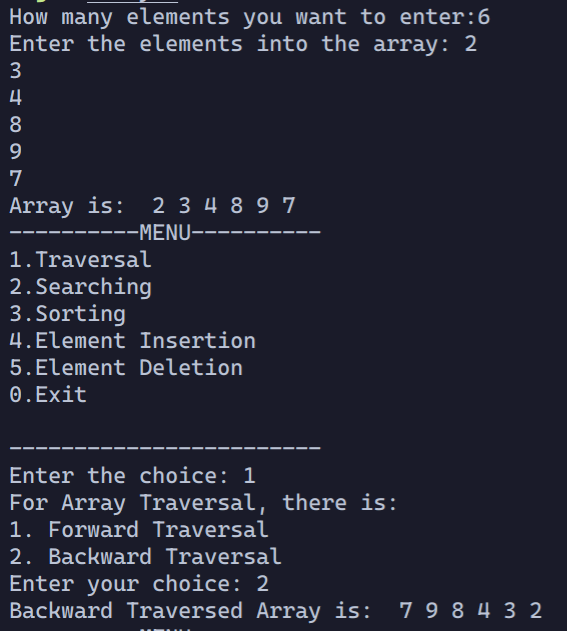
\includegraphics[width=110mm,scale=0.5]{../Array/outputs/array.png}

% -------------------Linked List----------------------------%

\chapter{Singly Linked List}
\section{Create a program of Singly Linked List and implement the following options:} 
\begin{center}
  ------------------- \\
            MENU \\
  ------------------- \\
  \begin{varwidth}{\textwidth}
    \begin{itemize}
      \item  \textbf {Create a node}
      \item  \textbf {Insert node}
      \begin{enumerate}[label=(\Roman*)]
        \item Insert at first
        \item Insert at the end
        \item Insert between the nodes 
      \end{enumerate}
      \item  \textbf {Delete a Node}
      \item \begin{enumerate}[label=(\Roman*)]
        \item Delete at first
        \item Delete at the end
        \item Delete between the nodes 
      \end{enumerate}
      \item  \textbf {Count Number of Nodes}
      \item  \textbf {Print the Linked List}
      \item  \textbf {Reverse the Linked List}
      \item  \textbf {Exit}
    \end{itemize}
    ------------------- \\
  \end{varwidth}
\end{center}   
\bigbreak
\underline{\emph{\Large Source Code :}}
\inputminted[breaklines]{c}{../Linked_List/singly_linked_list.c}
\bigbreak
\noindent
\underline{\emph{\Large Program Output :}}
\bigbreak
\noindent
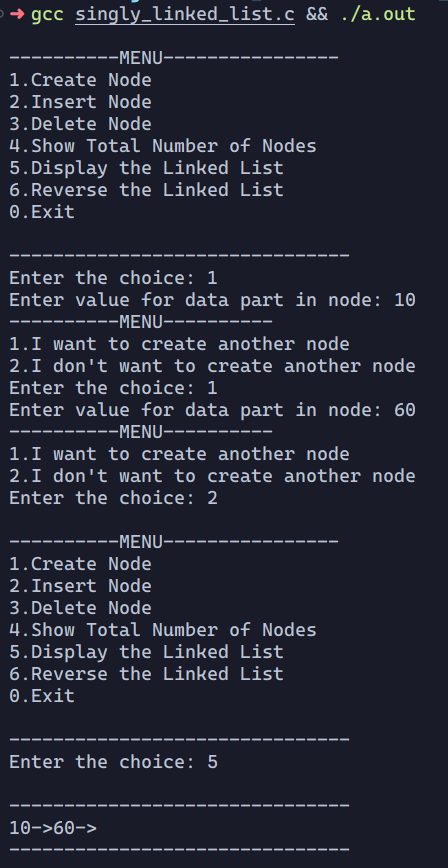
\includegraphics[width=110mm,scale=0.5]{../Linked_List/outputs/sll.png}

\chapter{Doubly Linked List}
\section{Work In Progress :)} 

\end{document}

